\chapter{Netio3}
\label{chap:netio3}

Netio3 \cite{netio3-docs} is a transport-agnostic networking library originally created for the Phase-2 \acs{FELIX} system, offering both TCP and \acs{RDMA} communication pathways.  It is organized into two modules: the \texttt{netio3-backend} and the \texttt{netio3-frontend}.  The backend is responsible for data transmission and reception over the network and does not contain any \acs{FELIX}-specific logic, making it reusable in other projects. The frontend builds on this by providing buffered I/O for data coalescence, a publish/subscribe API and data formatting.  Under the hood, TCP transport is implemented by the \acs{ATLAS} \acs{T-DAQ} \texttt{asyncmsg} \cite{asyncmsg} library, while \acs{RDMA} operations use the \texttt{libfabric} \cite{libfabric} library.  Both transports follow a connection-oriented, message-based paradigm.

\section{Netio3 backend}

Both the \texttt{asyncmsg} and the \texttt{libfabric} backend are implemented with the \emph{Reactor} design pattern, by using an event-driven model in the form of an event loop. Events can be callbacks from the underlying network library notifying the application about new connections, incoming data or user defined callbacks added through signals and timers. The event loop is single threaded, thus guaranteeing that all events are executed sequentially. Each event is associated with a callback that contains the user code that is executed when the event is triggered.

\subsection{Eventloop implementation}

There are two different event loop implementations: One based on the Linux kernel epoll system call (EpollEventLoop), and one based on \texttt{Boost::ASIO::io\_service} (AsioEventLoop). Both backends (The two versions are described below) are compatible with either event loop implementation. The same event loop can be used to power multiple backends.


\subsection{Libfabric backend}
\label{subsec:libfabric}

\texttt{libfabric} \cite{libfabric} is a library that provides a high-performance, low-latency communication interface for distributed applications. It abstracts the underlying network hardware and protocols, allowing developers to write portable code that can run on different network technologies without worrying about the specifics of the network stack. \texttt{libfabric} is especially useful when there are multiple systems using different network hardware and protocols, like in \acs{ATLAS}, because without it, one would to write separate code for each network type; instead \texttt{libfabric} offers a programming interface called the OpenFabrics Interfaces (OFI). When an application wants to send data, it makes calls to \texttt{libfabric} using this standard interface. \texttt{libfabric} then translates these calls into the specific commands needed for whatever network hardware is actually installed in the system. The library supports various transport protocols, including TCP and \acs{RDMA}.

\subsubsection{Sending data}

One way to achieve high performance is to avoid data copies. This is done by registering memory regions with an \acs{RDMA} device. Memory registration is an operation that pins\footnote{pinning a memory region means that the operating system will not move that data to different physical locations or swap it to disk.} that memory region only for an \acs{RDMA} device, since sending data to an \acs{RDMA} device from outside registered memory regions is not possible. The real advantage of RDMA is that the network hardware can directly access physical memory addresses (both for reading and writing), bypassing the CPU entirely for data transfers.\\

For \texttt{buffered sending}, a given number of buffers is allocated in memory, and registered with \texttt{libfabric}.\\
For memory coherency and to avoid data corruption, a buffer can never be modified after send\_buffer is called and before receiving the completion message. Matching send operations with completions is done internally.

For \texttt{zero-copy sending}, two memory regions are registered: one main memory region containing the data, and one region containing the additional header information (a completion object of 16 bytes per send operation).  Matching the send operations with completions is not supported by the library and has to be managed by the user.

\subsubsection{Receiving data}

As for sending data, receiving data also requires registering memory regions. When data is received, it is placed into an available buffer by the \acl{NIC} and provided to the user via a receive-completion callback. After reading, the buffer is then returned to the \texttt{libfabric} backend and can be used for the next receive operation.\\
For the \texttt{libfabric} backend, opening and closing connections is an expensive operation.

\subsection{Asyncmsg backend}
\label{subsec:asyncmsg}

\texttt{asyncmsg} is a message based wrapper of \texttt{Boost::ASIO}, developed by the \acs{ATLAS} \acs{T-DAQ} group. It provides a high-level interface for asynchronous message passing over TCP/IP networks, allowing applications to send and receive non-blocking messages (what asynchronous means).\\
The \texttt{asyncmsg} backend is thread safe.

\subsubsection{Sending data}

Contrary to the \texttt{libfabric} backend, the data for zero-copy sending in \texttt{asyncmsg} does not have to reside inside a registered memory region.\\
The most practical feature of \texttt{asyncmsg} for sending data is \texttt{immediate sending}, which essentially copies the data into a dynamically allocated buffer and sends it right away. This method does not require the allocation of multiple buffers, imposes no restrictions on data size, and does not require the user to guarantee data stability. However, it is also the slowest method of data transmission. For applications requiring high performance, the \texttt{libfabric} backend is preferred.

\subsubsection{Receiving data}

Also for receiving data the user is not required to register memory regions, thus reducing the memory footprint of the applications. This advantage comes at the cost of performance.\\

\section{Netio3 Frontend}

The netio3 frontend is built on top of netio3 backend to handle communications in a distributed system for data acquisition. The frontend introduces features such as data coalescence, a publish/subscribe \acs{API}, and a buffer formatting mechanism.

\textbf{Data Coalescence} is one of the core features provided by the netio3 frontend, which consists of a buffering layer that aggregates multiple small messages into larger network packets.\\
This feature is useful in scenarios with bursty or fine-grained message patterns, as it averages the cost of network transmission over multiple messages.


\section{Personal Contributions}

\subsection{New network buffer format}

The \texttt{felix-star} application processes uplink data by dividing it into 1\,KB \texttt{blocks}, decoding these blocks, and passing the decoded data to \texttt{netio3}, which adds a header for the remote clients. 
Previously, a fixed 13-byte header was used; for messages of 10 bytes (or smaller), the overhead ratio was inefficient.
The enhancement involved designing a new, more efficient header and updating the encode/decode routines accordingly \cite{netio3-header-commit}.\\

\begin{figure}[htbp]
\centering
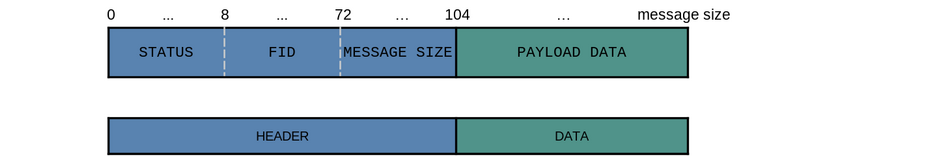
\includegraphics[width=\textwidth]{images/contributions/old-buffer-format.png}
\caption[Legacy format of network buffer]{Legacy buffer format with a 13-byte header. The numbers shown on top are bits}
\label{fig:old-buffer-format}
\end{figure}

\begin{figure}[htbp]
\centering
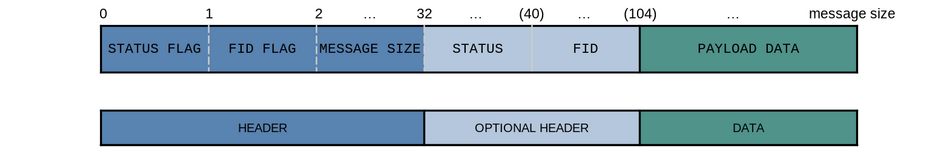
\includegraphics[width=\textwidth]{images/contributions/new-buffer-format.png}
\caption[New network buffer format]{Revised buffer format, reducing header overhead. The numbers shown on top are bits.}
\label{fig:new-buffer-format}
\end{figure}

This optimization works because data in the same \texttt{block} is guaranteed to have the same \acs{FID} since a \texttt{block} is encoded with data coming only from one \acs{E-link}.\\
See Figure~\ref{fig:block-format} to recall the \texttt{block} format that helps follow the next calculations.\\
Supposing the \texttt{block} is filled, to be conservative with the size, messages of 26 bytes, which is bigger than the size of a typical message coming from \acs{ITk}. A \texttt{block}, as shown in Figure~\ref{fig:block-format} has always a block-header of 4 bytes (32 bits), and for every other message (\texttt{chunks} and \texttt{subchunks}) there is a header of 4 bytes.

We calculate the number of total 26-byte \texttt{chunks} that fit into a \texttt{block} using:

\[
\frac{1024~\text{bytes} - 4~\text{bytes}}{26~\text{bytes} + 4~\text{bytes}} = 34~\text{chunks}
\]

Generalizing this:

\[
\frac{\text{block size} - \text{block header}}{\text{chunk size} + \text{chunk header}} = \text{number of chunks in a block}
\]

We determined that 34 chunks fit into a block. Now, we compute how much space they occupy in the network buffer using both the old and new buffer formatting schemes.

\paragraph{Old Buffer Format}

Each chunk is preceded by a 13-byte header, so:

\[
(13~\text{bytes} + 26~\text{bytes}) \cdot 34 = 1326~\text{bytes}
\]

\paragraph{New Buffer Format}

The first chunk has a full header:

\[
13~\text{bytes} + 26~\text{bytes} = 39~\text{bytes}
\]

The remaining 33 chunks share the same \ac{FID} and only require a 4-byte header each:

\[
(4~\text{bytes} + 26~\text{bytes}) \cdot 33 = 990~\text{bytes}
\]

Total buffer occupancy:

\[
39~\text{bytes} + 990~\text{bytes} = 1029~\text{bytes}
\]

In a conservative scenario with the new formatting, the network buffer would fit $\approx$\text{25\%} more messages.